% title: 벤 다이어그램 (교집합)
% description: 전체집합 U 안의 두 집합 A, B. 교집합 A ∩ B를 색칠한다
% packages:
% libraries:
% \R(반지름), \dist(두 중심 사이 거리)만 바꾼다. 색칠할 영역은 scope 안의 \clip과 \fill로 정한다.
% 합집합: scope 없이 두 원을 \fill. 차집합 A - B: \fill(A) 다음 \fill[white](B) 후 테두리를 다시 그린다.
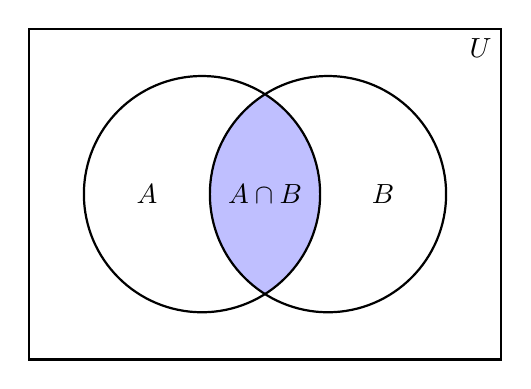
\begin{tikzpicture}
  \def\R{1.5}
  \def\dist{1.6}
  \coordinate (A) at (0,0);
  \coordinate (B) at (\dist,0);
  \begin{scope}
    \clip (A) circle[radius=\R];
    \fill[blue!25] (B) circle[radius=\R];
  \end{scope}
  \draw[thick] (A) circle[radius=\R] (B) circle[radius=\R];
  \draw[thick] (-\R-0.7,-\R-0.6) rectangle (\dist+\R+0.7,\R+0.6);
  \node at ({\dist/2-\R},0) {$A$};
  \node at ({\dist/2+\R},0) {$B$};
  \node at ({\dist/2},0) {$A\cap B$};
  \node[below left] at (\dist+\R+0.7,\R+0.6) {$U$};
\end{tikzpicture}
